\documentclass[journal]{IEEEtran}

\usepackage{amsmath,amssymb}
\usepackage{graphicx}
\usepackage{booktabs}
\usepackage{cite}
\usepackage{hyperref}
\usepackage{textcomp}

\graphicspath{{./figures/}}

\hyphenation{}

\begin{document}

\title{Learning the GHZ Game with Multi-Agent Reinforcement Learning}

\author{Xiangdong~Zheng~\IEEEmembership{ }

\thanks{Xiangdong Zheng is with the School of Information and Communication
        Engineering, University of Electronic Science and Technology of China
        (UESTC), Chengdu, China. E-mail: zx.dong@std.uestc.edu.cn.}
}

\maketitle

\begin{abstract}
The Greenberger--Horne--Zeilinger (GHZ) game is a three-player cooperative game in which any classical strategy achieves a win rate of at most 75\%, while a quantum strategy based on a shared GHZ entangled state achieves 100\%. This work investigates whether multi-agent deep reinforcement learning can autonomously discover an optimal classical strategy. We formulate the GHZ game as a cooperative multi-agent Markov game and train agents using Multi-Agent Proximal Policy Optimization (MAPPO) with a shared policy network conditioned on agent identity. Over five independent random seeds, the agents converge to the 75\% classical bound in three seeds, while the remaining two remain stuck at a suboptimal random-play equilibrium---a stationary point induced by the parity structure of the game. Ablation experiments indicate that network capacity, in particular the agent-identity embedding dimension, is the critical factor for convergence, whereas a centralized critic and entropy decay are helpful but not essential. We complement the learning experiments with an explicit Born-rule calculation of the GHZ-state quantum strategy, which confirms the 100\% win rate and illustrates the interference-driven cancellation of all losing outcomes.
\end{abstract}

\begin{IEEEkeywords}
multi-agent reinforcement learning, MAPPO, GHZ game, quantum advantage, entanglement
\end{IEEEkeywords}

\section{Introduction}

\IEEEPARstart{T}{he} GHZ game, introduced by Greenberger, Horne, and Zeilinger~\cite{ghz1989}, is a canonical example of quantum pseudo-telepathy: a task that can be solved perfectly using quantum entanglement but admits only a limited success rate under classical resources. Three players---Alice, Bob, and Carol---are each given a letter X or Y by a referee. The total number of X's is always odd (XXX, XYY, YXY, or YYX). Each player replies $+$ or $-$ without communication. The team wins if the number of $+$ replies is odd in scenario XXX and even in the other three scenarios.

A simple parity argument shows that no classical strategy can win all four scenarios: the four win-condition equations multiply to $1 = -1$, so at most three can be satisfied~\cite{mermin1990mysteries}. The resulting classical bound is 75\%. If the players instead share a three-qubit GHZ state $(|000\rangle + |111\rangle)/\sqrt{2}$ before the game and measure in appropriately chosen bases, quantum interference cancels every losing outcome, yielding a 100\% win rate~\cite{mermin1990extreme,brassard2003}.

The game-theoretic analysis of the GHZ game is well established. This paper addresses a different question: can autonomous agents, trained purely through trial and error, discover the optimal classical strategy without any prior knowledge? The problem sits at the intersection of multi-agent reinforcement learning (MARL) and quantum foundations~\cite{gronauer2022marl}. Despite its simplicity---four scenarios, two actions per agent, single-step episodes---it presents non-trivial coordination challenges.

We apply Multi-Agent Proximal Policy Optimization (MAPPO)~\cite{yu2022mappo}, with a shared policy network conditioned on learnable agent-identity embeddings. Our main findings are summarized below. First, MAPPO agents converge to the 75\% classical bound in a majority of random seeds, learning a deterministic ``all output $-$'' policy that wins three of four scenarios. Second, we identify a systematic failure mode in which the uniform random policy constitutes a suboptimal stationary point in the joint policy space, trapping gradient-based methods in 2 of 5 seeds and in a small-network ablation. Third, ablation experiments show that the agent-identity embedding dimension is the critical architectural choice; a centralized critic and entropy decay improve training stability but are not strictly necessary for convergence under favorable initializations.

\section{Background}

\subsection{The GHZ Game and the Classical Bound}

The game involves three players $i \in \{0,1,2\}$ and a referee. The referee selects a scenario $s \in \mathcal{S} = \{\text{XXX}, \text{XYY}, \text{YXY}, \text{YYX}\}$ uniformly at random. Player $i$ privately observes $o_i \in \{X, Y\}$ and outputs $a_i \in \{+, -\}$. The team wins if
\begin{equation}
    n_+ \equiv \begin{cases}
        1 \pmod{2}, & s = \text{XXX} \\
        0 \pmod{2}, & \text{otherwise}
    \end{cases}
\end{equation}
where $n_+ = |\{i : a_i = +\}|$.

The 75\% upper bound follows from a parity argument~\cite{mermin1990mysteries}. Let $f_i(o) \in \{+1, -1\}$ be the deterministic response of player $i$ to observation $o$, where $+1$ denotes $+$ and $-1$ denotes $-$. The product $f_0(o_0) f_1(o_1) f_2(o_2)$ equals $+1$ if the number of $+$ responses is even and $-1$ if odd. The four win conditions become:
\begin{align}
    f_0(X) f_1(X) f_2(X) &= +1 \label{eq:c1} \\
    f_0(X) f_1(Y) f_2(Y) &= +1 \label{eq:c2} \\
    f_0(Y) f_1(X) f_2(Y) &= +1 \label{eq:c3} \\
    f_0(Y) f_1(Y) f_2(X) &= +1 \label{eq:c4}
\end{align}
Multiplying (\ref{eq:c1})--(\ref{eq:c4}), each $f_i(o)$ appears exactly twice on the left-hand side, giving $(f_i(o))^2 = +1$. The product of the four left-hand sides is $+1$. The product of the four right-hand sides is $(-1) \cdot (+1)^3 = -1$. The contradiction $+1 = -1$ proves that no assignment of $\pm 1$ to the six variables $\{f_i(X), f_i(Y)\}_{i=0}^2$ can satisfy all four equations. At most three can hold simultaneously, so the win rate is bounded by $3/4$. This deterministic bound extends to stochastic strategies by convexity: any mixed strategy is a convex combination of deterministic ones, each earning at most $3/4$, so the expected win rate cannot exceed $3/4$.

All optimal classical strategies share a particular structure. From (\ref{eq:c1})--(\ref{eq:c4}), if the first three equations are satisfied, the fourth must be violated. Inspecting the equations, one class of optimal strategies sets all six $f_i(o) = +1$ (all players always output $+$) or all $f_i(o) = -1$ (all players always output $-$). Under ``all $-$'', $n_+ = 0$ in every scenario, which is even, so XXX (which requires odd $n_+$) is lost. Any permutation where all three agents always output the same sign is equivalent and optimal.

\subsection{Quantum Strategy}

If the players share the GHZ state
\begin{equation}
    |\text{GHZ}\rangle = \frac{1}{\sqrt{2}}\bigl(|000\rangle + |111\rangle\bigr)
\end{equation}
before the game, they can exceed the classical bound~\cite{brassard2003}. Quantum optimization techniques have recently been explored for resource orchestration in networked systems~\cite{zheng2025power}. The quantum protocol is: on receiving $X$, measure in the Pauli-$X$ basis $\{|+\rangle, |-\rangle\}$; on receiving $Y$, measure in the Pauli-$Y$ basis $\{|+i\rangle, |-i\rangle\}$. The measurement outcome ($+$ or $-$) is the answer of the player.

The Born-rule probability of outcome $(a,b,c)$ is
\begin{equation}
    P(a,b,c) = \bigl|\langle \psi_a| \otimes \langle \psi_b| \otimes \langle \psi_c| \; |\text{GHZ}\rangle \bigr|^2
\end{equation}
where $|\psi_a\rangle$ is the eigenstate for outcome $a$ in the prescribed basis. Concretely, $\langle +|0\rangle = \langle -|0\rangle = 1/\sqrt{2}$, $\langle +|1\rangle = 1/\sqrt{2}$, $\langle -|1\rangle = -1/\sqrt{2}$ for the X basis; similarly, $\langle +i|0\rangle = 1/\sqrt{2}$, $\langle +i|1\rangle = i/\sqrt{2}$, $\langle -i|0\rangle = 1/\sqrt{2}$, $\langle -i|1\rangle = -i/\sqrt{2}$ for the Y basis.

In scenario XXX where all three measure in the X basis, the amplitude for outcome $(a,b,c)$ expands to
\begin{equation}
    \langle abc|\text{GHZ}\rangle = \frac{1}{2}\bigl(\langle a|0\rangle\langle b|0\rangle\langle c|0\rangle + \langle a|1\rangle\langle b|1\rangle\langle c|1\rangle\bigr).
\end{equation}
The two terms have equal magnitude. When the number of $+$ outcomes is even, the product $\langle a|0\rangle\langle b|0\rangle\langle c|0\rangle$ equals $-\langle a|1\rangle\langle b|1\rangle\langle c|1\rangle$, producing exact cancellation. When the number of $+$ is odd, the two terms are equal, yielding constructive interference. An analogous argument holds for scenarios involving Y measurements, where the relative phase factors of $\pm i$ from the Y-basis states produce the same pattern of cancellation for odd-$n_+$ outcomes. In each scenario, four of the eight outcomes have zero amplitude, and the four surviving outcomes all satisfy the win condition with equal probability $1/4$, giving a win probability of 1.

\subsection{Multi-Agent Formulation}

We model the GHZ game as a cooperative multi-agent Markov game with a single time step per episode. The observation for each agent is $o_i \in \{0, 1\}$, with 0 encoding X and 1 encoding Y. The action space is $a_i \in \{0, 1\}$, where $0 = +$ and $1 = -$. The reward is $R = +1$ for a win and $-1$ for a loss, shared identically across all agents. The objective is to maximize the expected win rate over the uniform distribution of scenarios. Because each episode is a single step, this formulation is equivalent to a multi-agent contextual bandit with cooperative rewards and no communication.

\section{Method}

\subsection{Architecture}

We use the MAPPO framework~\cite{yu2022mappo} with centralized training and decentralized execution (CTDE).

\textbf{Shared actor with agent-ID embedding.} All three agents share a single policy network $\pi_\theta(a \mid o, \text{id})$. Each agent $i$ is assigned a learnable embedding vector $\mathbf{e}_i \in \mathbb{R}^4$. The actor is a two-hidden-layer MLP (32 units per layer, ReLU) that takes the concatenation $[o_i \parallel \mathbf{e}_i]$ as input and outputs action logits. Parameter sharing is sample-efficient, while the identity embedding allows role differentiation.

\textbf{Centralized critic.} The critic $V_\phi(\mathbf{o})$ is a two-hidden-layer MLP (64 units per layer, ReLU) that takes the concatenated observations of all three agents as input. During training, the critic sees the full joint state, reducing credit-assignment variance. At execution, only the decentralized actor is used.

\subsection{Training}

The training procedure follows the standard policy gradient framework~\cite{sutton2018book} using PPO~\cite{schulman2017ppo}. For each episode (a single game step), the advantage is
\begin{equation}
    \hat{A} = R - V_\phi(\mathbf{o})
\end{equation}
and is normalized to zero mean and unit variance over the batch of 256 episodes. The actor loss is the clipped surrogate objective:
\begin{equation}
    \mathcal{L}^{\text{actor}} = -\mathbb{E}\Bigl[\min\bigl(r(\theta)\hat{A},\; \text{clip}(r(\theta), 1-\epsilon, 1+\epsilon)\hat{A}\bigr) - \beta H(\pi_\theta)\Bigr]
\end{equation}
where $r(\theta) = \pi_\theta(a|o) / \pi_{\theta_{\text{old}}}(a|o)$, $\epsilon = 0.2$, and $H$ is the policy entropy. The critic is updated via MSE: $\mathcal{L}^{\text{critic}} = (V_\phi(\mathbf{o}) - R)^2$.

After every 256 episodes, the buffer is used for 8 PPO epochs with mini-batches of size 256. The entropy coefficient $\beta$ starts at 0.05 and decays by factor 0.95 per update (lower-bounded at 0.001). The learning rate decays by factor 0.98 per update from $10^{-3}$. Gradients are clipped to norm 0.5. Training runs for 15,000 episodes. Table~\ref{tab:hyper} lists all hyperparameters.

\begin{table}[!t]
\centering
\caption{Hyperparameters.\label{tab:hyper}}
\begin{tabular}{@{}ll@{}}
\toprule
\textbf{Parameter} & \textbf{Value} \\
\midrule
Agents                  & 3 \\
Actor hidden dim        & 32 \\
Critic hidden dim       & 64 \\
Agent-ID embedding dim  & 4 \\
PPO clipping $\epsilon$ & 0.2 \\
Entropy coefficient $\beta$ & 0.05 $\to$ 0.001 \\
Entropy decay factor    & 0.95 (per update) \\
Learning rate           & $10^{-3}$ \\
LR decay factor         & 0.98 (per update) \\
PPO epochs per update   & 8 \\
Batch / mini-batch size & 256 \\
Max gradient norm       & 0.5 \\
Training episodes       & 15,000 \\
\bottomrule
\end{tabular}
\end{table}

\section{Experiments}

We conduct four sets of experiments: (i) multi-seed convergence, (ii) training dynamics and policy analysis, (iii) ablation studies, and (iv) quantum simulation.

\subsection{Convergence Across Random Seeds}

We train the MAPPO agents on five independent random seeds (42, 123, 456, 789, 1024). Fig.~\ref{fig:training} shows training curves.

\begin{figure}[!t]
    \centering
    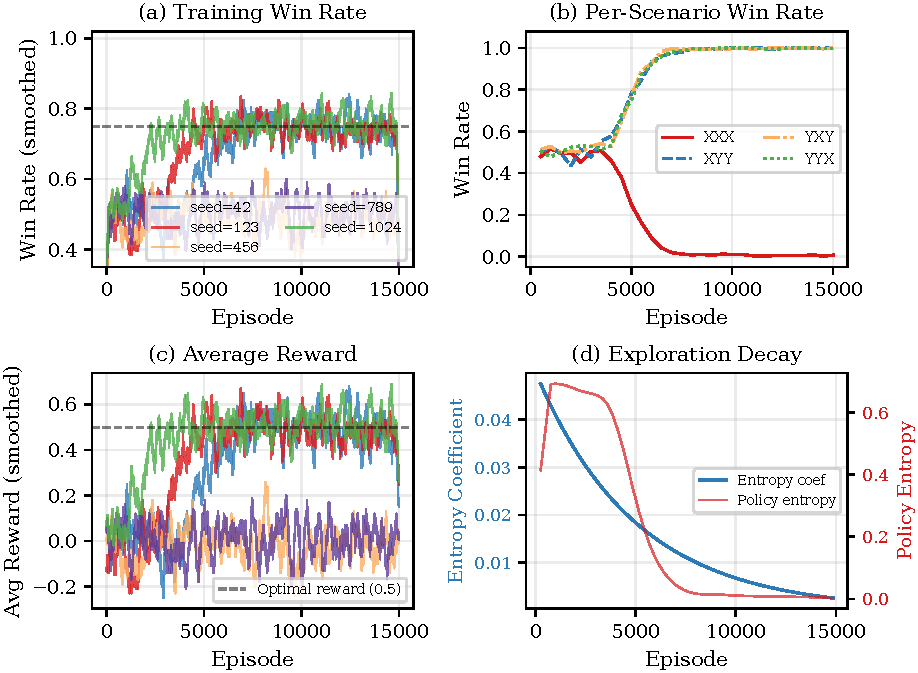
\includegraphics[width=\columnwidth]{fig2_training_dynamics.pdf}
    \caption{Training dynamics. (a) Smoothed training win rate for five seeds, with the dashed line at 0.75. (b) Per-scenario evaluation win rate (seed 42). (c) Smoothed average reward. (d) Entropy coefficient decay and policy entropy (seed 42).}
    \label{fig:training}
\end{figure}

Three of five seeds converge to the classical bound, with best evaluation win rates of 0.767, 0.765, and 0.774 (mean $0.769 \pm 0.004$ for converged seeds). The remaining two seeds (456, 789) remain near 0.50, equivalent to random play. Fig.~\ref{fig:multiseed} shows the mean and standard deviation across all seeds.

\begin{figure}[!t]
    \centering
    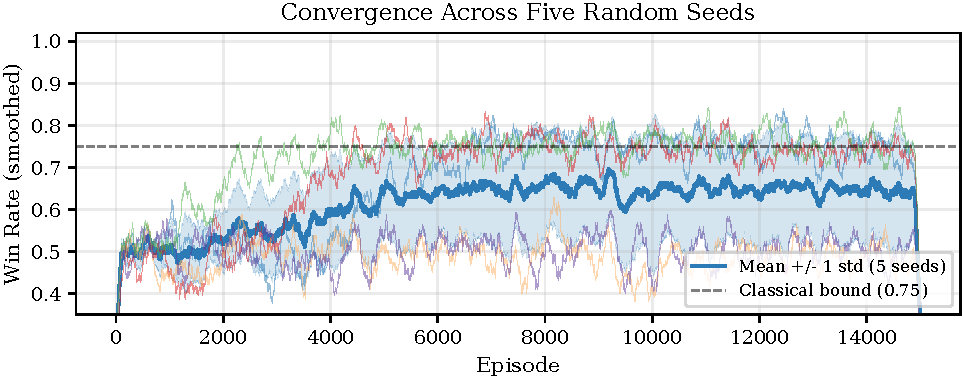
\includegraphics[width=\columnwidth]{fig7_multi_seed_summary.pdf}
    \caption{Mean win rate $\pm 1$ standard deviation over five seeds. The wide band reflects the divergence between converged and failed seeds.}
    \label{fig:multiseed}
\end{figure}

The per-scenario breakdown for seed 42 reveals the structure of the learned strategy: 100\% win rate on XYY, YXY, and YYX, and approximately 0\% on XXX. This matches the ``all $-$'' strategy: $n_+ = 0$ (even) wins all scenarios except XXX.

\subsection{Policy Evolution}

Fig.~\ref{fig:policy} traces the policy probabilities $P(+ \mid \text{observation})$ for each agent during training (seed 42). At episode 500, all three agents output $+$ with probability 0.5--0.6, reflecting the initial exploration regime. By episode 5,000, $P(+ \mid \cdot) < 0.3$ for all agents; by episode 10,000, $P(+) < 0.05$; and at episode 15,000, $P(+) < 0.002$ for all observation--agent combinations. The policy is essentially deterministic.

\begin{figure}[!t]
    \centering
    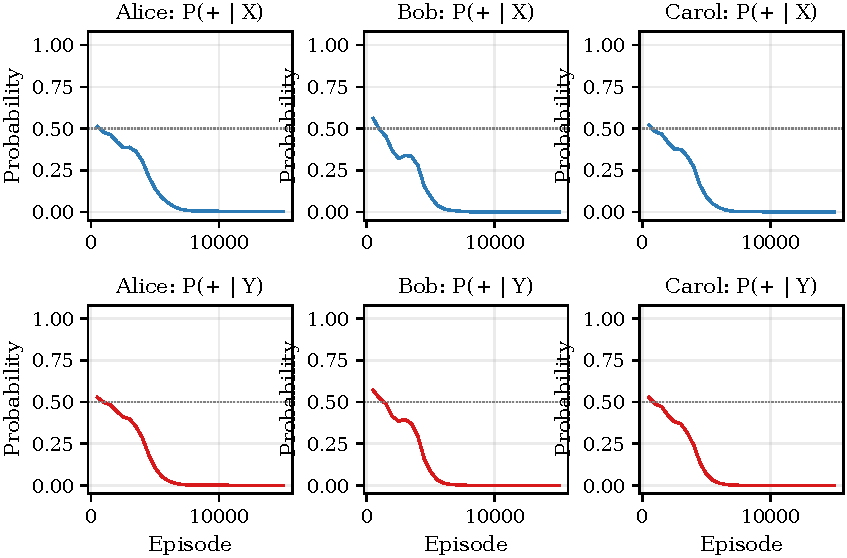
\includegraphics[width=\columnwidth]{fig3_policy_evolution.pdf}
    \caption{Policy probabilities $P(+ \mid X)$ (top) and $P(+ \mid Y)$ (bottom) for each agent during training (seed 42). All probabilities converge toward zero.}
    \label{fig:policy}
\end{figure}

The agents consistently converge to ``all $-$'' rather than the equivalent ``all $+$'' strategy. This asymmetry is determined by random weight initialization and the stochasticity of early training, not by any bias in the problem formulation.

\subsection{Ablation Studies}

We compare the baseline MAPPO against three variants, all using seed 42: (1) no entropy decay, with $\beta$ fixed at 0.05; (2) IPPO (independent critics), in which three separate critics each observe the input of a single agent; and (3) a small network, with the actor hidden dimension reduced from 32 to 16, the critic hidden dimension from 64 to 32, and the embedding dimension from 4 to 2.

\begin{figure}[!t]
    \centering
    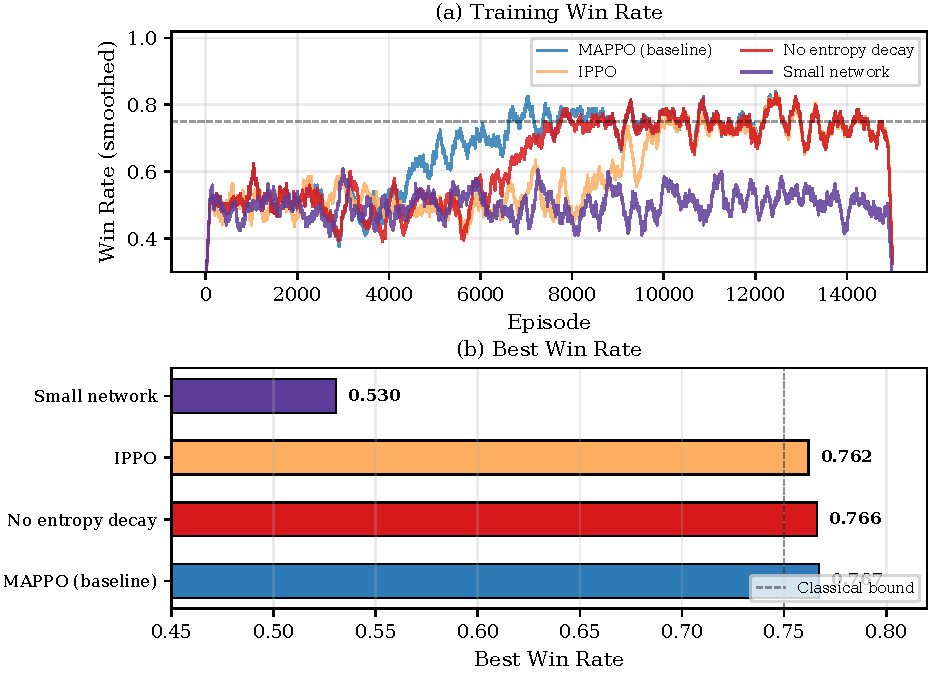
\includegraphics[width=\columnwidth]{fig6_ablations.pdf}
    \caption{Ablation results. (a) Smoothed training win rate. (b) Best evaluation win rate per variant.}
    \label{fig:ablations}
\end{figure}

Table~\ref{tab:ablation} summarizes the results. The baseline, no-entropy-decay, and IPPO variants all converge to approximately 0.76, indicating that neither entropy decay nor a centralized critic is strictly necessary for this problem when initialization is favorable. The small-network variant fails to exceed the random baseline, achieving only 0.531. Inspection shows the policy remains stochastic with $P(+) \approx 0.46$ for all agents. A 2-dimensional embedding appears insufficient to cleanly differentiate three agent identities.

\begin{table}[!t]
\centering
\caption{Ablation results (seed 42).\label{tab:ablation}}
\begin{tabular}{@{}lcc@{}}
\toprule
\textbf{Variant} & \textbf{Best WR} & \textbf{Converged} \\
\midrule
Baseline (MAPPO)       & 0.767 & Yes \\
No entropy decay       & 0.766 & Yes \\
IPPO (indep.\ critics) & 0.762 & Yes \\
Small network          & 0.531 & No \\
\bottomrule
\end{tabular}
\end{table}

\subsection{Quantum Simulation}

We compute the Born-rule probabilities for the GHZ-state strategy described in Section~II-B. In each scenario, exactly four of the eight outcome combinations have non-zero probability (0.25 each), and all four satisfy the win condition (Fig.~\ref{fig:qm}).

\begin{figure}[!t]
    \centering
    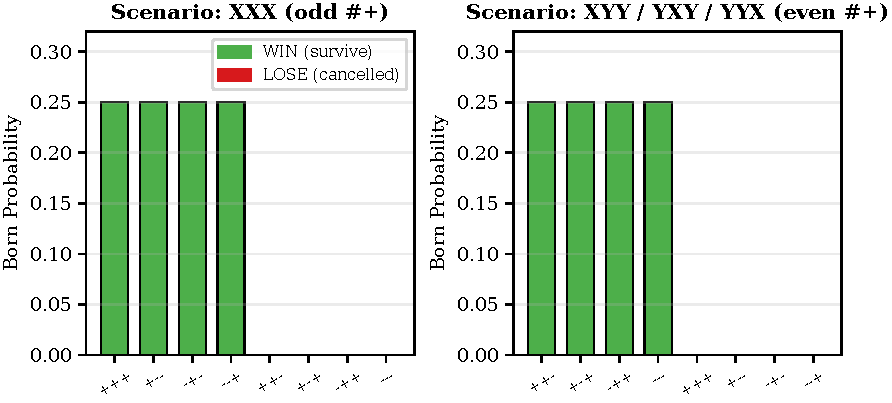
\includegraphics[width=\columnwidth]{fig5_quantum_interference.pdf}
    \caption{Born-rule probabilities for the XXX scenario (left) and XYY/YXY/YYX (right). Green bars: winning outcomes that survive interference (probability 0.25 each). Red bars: losing outcomes that are cancelled (probability 0).}
    \label{fig:qm}
\end{figure}

\begin{figure}[!t]
    \centering
    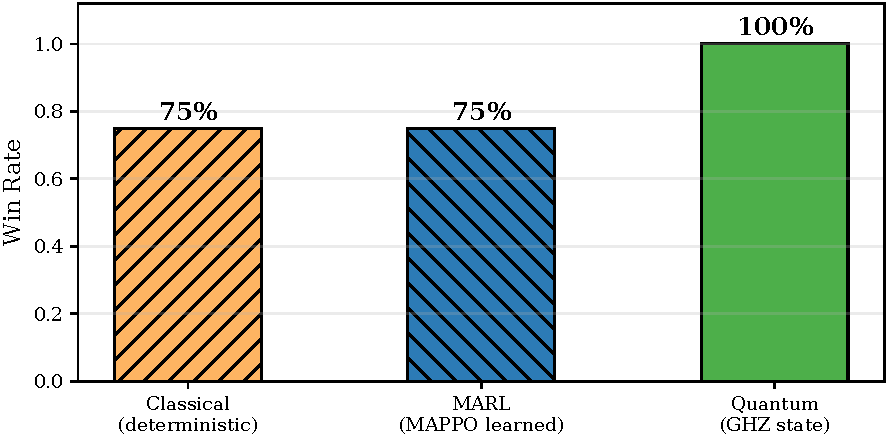
\includegraphics[width=\columnwidth]{fig4_quantum_vs_classical.pdf}
    \caption{Win rate comparison. Classical and MARL: 75\%; quantum GHZ strategy: 100\%.}
    \label{fig:qmbar}
\end{figure}

The overall quantum win rate is 100\% (Fig.~\ref{fig:qmbar}), representing a $+25$ percentage point advantage over the classical bound. The cancellation mechanism operates as follows: for XXX, the four outcomes with even $n_+$ are cancelled by destructive interference between the $|000\rangle$ and $|111\rangle$ components; for XYY/YXY/YYX, the four outcomes with odd $n_+$ are cancelled.

\subsection{Failure Mode Analysis}

The two failed seeds (456, 789) and the small-network ablation share a common failure pattern: all three agents maintain $P(+) \approx 0.5$ for both observations, equivalent to uniform random play, yielding a win rate of 0.50.

This behavior can be understood analytically. When all three agents use the uniform random policy, the expected reward is zero (half of scenarios won, half lost). For any single agent considering a deviation, the marginal benefit is also zero: if two agents are random, the action of the third agent does not affect the parity distribution. Formally, let $\pi_i(+ \mid o) = 0.5$ for all $i, o$. The expected return is
\begin{equation}
    J = \frac{1}{4}\sum_{s \in \mathcal{S}} \sum_{a_0,a_1,a_2} \pi_0(a_0|o_0)\pi_1(a_1|o_1)\pi_2(a_2|o_2) \cdot R(s, a_0, a_1, a_2).
\end{equation}
For any $i$, $\partial J / \partial \pi_i = 0$ because the marginal distribution over win/loss is uniform regardless of $\pi_i$ when the other two agents are uniform. The policy gradient therefore vanishes, creating a suboptimal stationary point. This is distinct from the standard single-agent exploration problem: the flat gradient is not due to insufficient exploration noise but to a structural property of the multi-agent payoff landscape.

Entropy decay is not the cause of failure---both failed seeds and the small-network variant use the same decay schedule as successful seeds. Instead, the random initialization determines which basin of attraction the policy falls into. In the random-play basin, the gradient signal is too weak to escape before entropy decays; in the successful basin, the initial policy is sufficiently asymmetric that the gradient drives it toward determinism.

This failure mode highlights a subtle challenge in cooperative MARL: even in seemingly trivial problems, the joint policy landscape can contain stationary points that trap gradient-based optimizers. The small-network variant is especially vulnerable because a 2-dimensional embedding provides limited capacity for the network to break symmetry among three agents during early training.

\section{Discussion}

\subsection{What Determines Success or Failure?}

The results suggest a hierarchy of factors. The most critical is network capacity: reducing the embedding dimension from 4 to 2 causes complete failure, as the embedding must provide sufficient representational capacity to distinguish three agent identities. Random initialization is also important, since some initializations place the policy in the basin of attraction of the random-play stationary point; with adequate capacity, this occurs in 2 of 5 seeds. A centralized critic has a moderate effect: IPPO converges (0.762 vs.\ 0.767 for MAPPO), but may require more careful tuning or additional episodes in harder settings. Entropy decay plays a minor role, as the no-entropy-decay variant converges successfully, confirming that the reward signal alone suffices to drive the policy toward determinism.

\subsection{Relation to Prior Work}

The GHZ game has been studied extensively in quantum foundations~\cite{ghz1989,mermin1990mysteries,mermin1990extreme,brassard2003}, but its intersection with reinforcement learning is relatively unexplored. Our work connects to the growing literature on MARL for cooperative games~\cite{yu2022mappo,lowe2017maddpg,rashid2018qmix,sunehag2018vdn}. The GHZ game serves as a minimal testbed for studying credit assignment in cooperative MARL: each agent receives identical rewards, and the coordination problem must be solved without communication.

The identification of the random-play stationary point as a failure mode relates to the broader challenge of local optima in multi-agent policy gradients~\cite{lowe2017maddpg,foerster2018coma}. Unlike standard single-agent RL, where entropy bonuses help escape local optima, the multi-agent setting can produce stationary points where no individual agent has an incentive to deviate.

\subsection{Limitations}

The GHZ game is a minimal problem (4 scenarios, 2 actions per agent), and the findings may not generalize to larger state-action spaces. We used MAPPO, a standard algorithm; more advanced methods such as QMIX~\cite{rashid2018qmix} or MAT~\cite{wen2022mat} may exhibit different behavior. Ablation experiments used a single seed (except the baseline), limiting statistical power. The failure mode analysis is primarily empirical; a formal characterization of the basin-of-attraction structure remains for future work.

\section{Conclusion}

We trained MAPPO agents to play the GHZ game and found that they converge to the optimal classical strategy (75\% win rate) in 3 of 5 random seeds. The learned strategy is a simple deterministic policy: every agent always outputs $-$. We identified a failure mode in which agents remain stuck at the random-play equilibrium, a suboptimal stationary point arising from the parity structure of the game. Ablation experiments showed that the agent-identity embedding dimension is critical, while entropy decay and a centralized critic are helpful but non-essential. We complemented the learning results with a Born-rule calculation of the quantum GHZ-state strategy, confirming the 100\% win rate and the interference-driven cancellation of losing outcomes.

Future work could apply MARL to more complex non-local games, such as the Mermin--Peres magic square~\cite{mermin1990simple,peres1990}; investigate whether agents can learn to exploit entanglement when quantum resources are made available in the action space; conduct a formal analysis of the policy landscape to better understand and mitigate the random-play stationary point; and explore whether value-decomposition methods exhibit different convergence behavior on this benchmark.

\appendices
\section{Game Schematic}

\begin{figure}[!t]
    \centering
    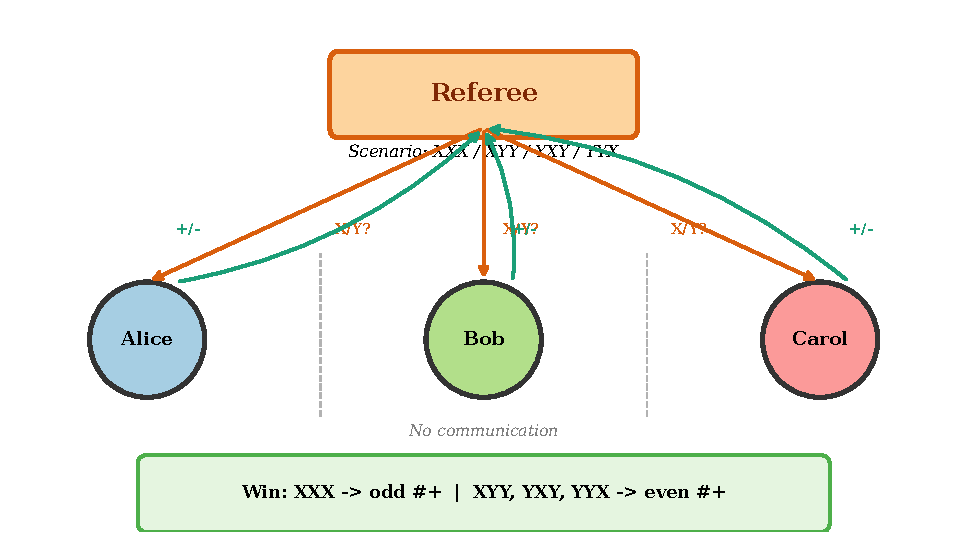
\includegraphics[width=\columnwidth]{fig1_game_schematic.pdf}
    \caption{Schematic of the GHZ game. A referee gives each player a letter (X or Y). Players reply $+$ or $-$ without communication. The win condition depends on the parity of $+$ responses.}
    \label{fig:schematic}
\end{figure}

\section*{Acknowledgment}
The authors thank [acknowledgments to be added].

\nocite{nielsen2010quantum,zheng2025power,zheng2024dual}
\bibliographystyle{IEEEtran}
\bibliography{ghz_marl}

\end{document}
